\documentstyle[cec2003,multicol,times,epsfig]{article}
% cec032e.tex, 23 Jan, 2003
%
% Example of using the cec2003.sty style file to prepare
% a paper for the 2003 Congress on Evolutionary Computation.
%

\begin{document}
\pagestyle{empty}
\sloppy

\twocolumn[
%
\title{Simme}
%
%% How you format the author information is up to you; this is
%% merely a suggestion:
%
\vspace{0.1in}
\vspace{0.25in}
] % end of the argument to \twocolumn

\begin{abstract}
Simme is a multiplayer game for mobile devices (mobile phones, PDAs, ...)
developed to provide a basis for a gaming forum in which new games can easily
be integrated. The architecture described in this document is targeted on
assisting the implementation of multiplayer games for mobile devices. 
\end{abstract}

\section{Introduction}
A lot of game developers, particulary developers working in the range of
wireless communication, are confronted with the same problem. Having a nice
game for 2 players, but the only chance to play the game, in multiplayer mode,
 on a mobile device is to share one device, because the costs of implementing
an autonomous server based version of the game are simply to high.\\
On the basis of this consideration the Simme project is trying to create a
platform in which a serverbased multiplayer version of an existing game can be
created with minimal effort.\\
Because of the strict parting of gamelogic and communication between Client and
Server we achieved, that on the server side of the game, only the communication
protocol between Client and Server (or rather between the two clients) has to be
implemented. 

\subsection{Description of the game Simme}

Simme is a game based on the Ramsey-theorem, describing the party puzzle, a
special case of the Ramsey theory. The Gameboard consists of six
points arranged in an hexagon, each linked the other five points. Alternately
the players set a connection between two points.\\
The player with the first complete triangle of connections looses the
game.\medskip

\begin{figure}[h]
\begin{center}
\epsfig{file=./pics/gameboard1.png, scale = 1}
\caption{Gameboard of Simme}
\end{center}
\end{figure}

The game can never end in a draw, there is always a winner. Due to the odd
number of connections between the vertexes of the hexagon, there can never be a
stalemate.\\
A close analysis of this game and the underlying Ramsey theory was done in the
paper "Graph Ramsey games" by Univ.-Prof.
Dipl.-Ing. Dr.techn. Wolfgang Slany \cite{slany_paper}.

The game was designed for mobile phones either to play against the
computer, or to play against another human player over the web. Therefor the
game was designed as a server-client game as described in the Architecture
section.

\section{Present Development State}
Until now the game Simme was implemented in the following versions:\\
\noindent as \textit{one player game (against a computer opponent)}, as
\textit{local multiplayer game (two players - one device)} and as
\textit{multiplayer game (with an external game server)}.\\
The main focus layed on the strict isolation of client and server, to design
game logic and communication between client and server as modular as possible,
for a good reusability for other games. \\
A close look on the architecture follows in section \ref{Architecture}.

\begin{enumerate}
\item \textit{one player game (against a computer opponent)}\\
A computer opponent is implemented. As described in section \ref{CI} at this
time there is no \textit{intelligent} computer opponent integrated in the game
Simme, but an opponent taking randomised turns.\\
The portation of a learning computer opponent, implemented as a Java-Applet
Version of the game (called HEXI) from Univ.-Prof.
Dipl.-Ing. Dr.techn. Wolfgang Slany, is planned \cite{slany_paper}.

\item \textit{local multiplayer game (two players - one device)}\\
In this Version of the game Simme two players play local against each other.
They share one mobile device an take turns one after the other.\\
A local multiplayer game Version will be the starting point for implementing
a server based version of other games in the future.

\item \textit{multiplayer game (with an external game server)}\\
This Version of the game is using the design described in section
\ref{Architecture}. Two human players are connecting to a game server, using
their mobile device, which controls the communication between the two players
and checks the data content.
\end{enumerate} 

With these three game layouts the porting of an existing game onto the
Simme-platform can be described.\\

\section{Going online} \label{going_online} 
Starting from a game - a local multiplayer game (Point 1 and 2 of the Present
Development State) - it's easy to implement the communikation between two
clients using an external server.\\
The task is to create an interface used by the server and the client to
communicate with each oter.\\

In which way can this interface be built? The Simme-server provides some base
classes, supporting the communication for 2 player-games. Using the protocol,
given by the Simme-server, the realisation of a serverbased multiplayer version
of a game is no problem any longer.

At the client side of the game there are just a few modifications to realise.
An interface has to be implemented which has to wait for turns, sent by the
game server. Besides this no other changes have to be done, no alterations in
the game logic or the game-flow have to be done.

\begin{figure}[h]
\begin{center}
\epsfig{file=./pics/internal_interface.png, scale=0.6}
\caption{Internal Interface}
\end{center}
\end{figure}


\section{Design Architecture} \label{Architecture}
As already said in section \ref{going_online}, the game server can be seen an
sole mediator between the game clients. The server has no access to the game
logic. Merely syntax checks can be carried out by the server on the Files and
requests sent by client and server.

\subsection{Advantages of the separation of server and gamelogic}
Because of the separation of the game logic from the server, the server is
nothing more than a link between the two players. All game internal check-ups
are done by the clients and so the server is not charged.\\
Further on its guaranteed that no \textit{needless information} is transferred.
For example an illegal game turn is not transferred to the server, because the
validation of moves is done in the clients. So the illegal turn will never
arrive at the server or the second player. \\

\subsection{Communication between client and server}
The communication between Client and Server is working in two different ways.
on the one hand the clients are sending direct http-requests, on the oder hand
the server is sending XML-Files to the clients. The XML-Files, created by the
server, are mostly \textit{responses} to the client requests.

\begin{figure}[h]
\begin{center}
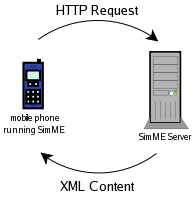
\epsfig{file=./pics/com_client_server.png, scale=0.5}
\caption{Communication between client and server}
\end{center}
\end{figure}

The communication interface exists of dynamic menues, created and administrated
by the game server. These dynamic menues can be reused by other games because
thea are organised in interface-classes and consequently are modular.

\subsection{Internal administration on the server}
The internal data organisation on the server side is carried out by means of a
database, containing informations about the games currently running and about
registered players. Further on with this database also the different games,
implemented on the Simme-platform, will be administrated.\\
Thus information about currently registered players, running games, and so on
can be obtained via SQL statements. \\
One of our next goals is to implement, alternatively to improve, the statistic
part of the database. In this way statistics about gaming behaviour, win-lose
statistics and much more can be implemented.

\section{Computational Intelligence} \label{CI}
At the present development state there is no implementation of a CI-gaming-unit
available on the Simme-server. The same game (also known under the name of
HEXI) was realised as a Java-Applet by Univ.-Prof. Dipl.-Ing. Dr.techn. Wolfgang
Slany. In this Version of the game, playable on
\textit{http://www.dbai.tuwien.ac.at/proj/ramsey/} a learning computer opponent
is implemented. You can take a closer look on the implementation of this
CI-gaming-unit in \cite{slany_paper}\\
\noindent Online version of this paper:\\
http://www.dbai.tuwien.ac.at/ftp/papers/slany/dbai-tr-99-34.ps.gz

\subsection{CI-Player for simme}
The CI-gaming-unit mentioned above will be integrated in the single player
version of the game Simme. On the client as on the server side. Through the
implementation of the CI-gamin-unit on the Simme-server we get the possibility
to record statistics about gaming strategies, because sole moves and therefor
whole game matches could be logically analysed. \\
Furtheron the learning CI-gaming-unit could even \textit{learn} from matches
played by two human players.\\
Based on these statistics an adjustment of gaming levels of the CI-gaming-unit
could be done, so to each player a CI-player with the same gaming level can be
assigned.\\


\section{Look-out on future developments}
In this section some ideas are listed we will implement in the future.

\subsection{Communication betwen the players during a running game}
Like Tony Manninnen says in "Interaction Forms and Communicative Actions in
Multiplayer Games"\cite{mann03}:
\begin{quotation}
Rich interaction is achieved through direct manipulation of
objects, multimodal input devices and the high number of degrees of freedom.
However, this
relatively technical definition covers only one portion of the concept. In
addition to these, social, cultural and communicative aspects have a significant
impact on interaction richness. [...]\\
\textit{Rich interaction does not necessarily require rich interfaces.}
\end{quotation} 
The last sentence of this quotation describes our approach to useful
communication forms between players really good. The idea is to provide some
\textit{hardcoded} Sentences which can be sent to the second player. In the
first place its a very time saving way to communicate in written form - which
is important because of the online costs of mobile devices - secondly, with fix
sentences, the possibility exists to use a database for translating these
sentences to different languages at a minimal cost.\\
Of course it is also planned to implement a chat functionality to aid a free
form of communication.

\subsection{Integration of the CI-gaming unit an the client and on the server}
Es described in \ref{CI} a CI-gaming-unit will be integrated in the
Simme-server on client side and on server side, to support a challenging sinple
player version one the one hand, and to improve the game statistics on the
other hand.\\
The CI-gaming-unit implemented by Dipl.-Ing. Dr.techn. Wolfgang Slany is a
lerning opponent, so the gamerecords will be used by the CI-gaming-unit to
improve the playing style.

\subsection{Improved game statistics}







\newpage


\begin{thebibliography}{10}
\bibitem[slany99]{slany_paper} Slany W. (1999) "Graph Ramsey games", Institut
f�r Informationssysteme Abteilung Datenbanken und Artificial Intelligence Technische
Universit�t Wien 
\bibitem[mann03]{mann03} Manninen T. (2003) "Interaction Forms and Communicative
Actions in Multiplayer Games",  The international journal of computer game
research

\end{thebibliography}

\end{document}
